\section{GUI-Fenster}
\label{guifenster0}

(Zum besseren Verständnis siehe \cref{windowclass})
Der Designer verfügt im allgemeinen drei Typen wie Seiten der GUI dargestellt werden können: Das Programm besitzt ein Hauptfenster, welches das Design von MahApps.Metro verwendet. (Siehe \cref{mahapps})
Dieses Hauptfenster kann nun in verschiedene Reiter unterteilt werden. Dies gehen wir mit der GUI Bibliothek DotNetBar (Siehe \cref{dotnetbar}) an.
Diese Reiter sind im Designer sogenannte \textit{Layouts}. Jeder der verschiedenen Layoutklassen stehen im Namespace \textit{FM3D\_Designer.src.WindowLayouts} und erben von der Klasse \textit{WindowLayout} im Namespace \textit{FM3D\_Designer.src}. Diese Klasse beinhaltet Attribute die jedes der Layouts verfügt. Die Klasse WindowLayout, welche wiederum von der Klasse \textit{DockWindow} der DotNetBar-Bibliothek erbt, sorgt dafür, dass die verschiedenen Seiten als Reiter und Unterfenster (oder auch child-windows) behandelt werden.
In jedem Layout ist es möglich verschiedene  kleinere Fenster aufzurufen. Der User kann diese Fenster innerhalb der Layouts oder des Desktops andocken. Jedes dieser \textit{ToolWindows} ist der Strukturierung wegen nochmal in einen weiteren Namespace unterteilt. Alle dieser \textit{ToolWindows} erben von der Klasse \textit{ToolWindow}, welche eine Initialisierungsmethode und eine Aggregation zu einem \textit{WindowLayout} verfügt.
Auch die Klasse \textit{ToolWindow} erbt von der Klasse \textit{DockWindows}.
Neben diesen Reitern und Unterfenstern verwendet der Designer noch sogenannte \textit{Dialoge}. All diese Dialoge erben von der Klasse \textit{DialogBase}, welche die Grundkomponenten der Dialoge beinhaltet. Diese Klasse erbt wiederum von \textit{BaseMetroDialog} welche sich in der MahApps.Metro Bibliothek befindet. 

\begin{figure}
	\begin{center}
		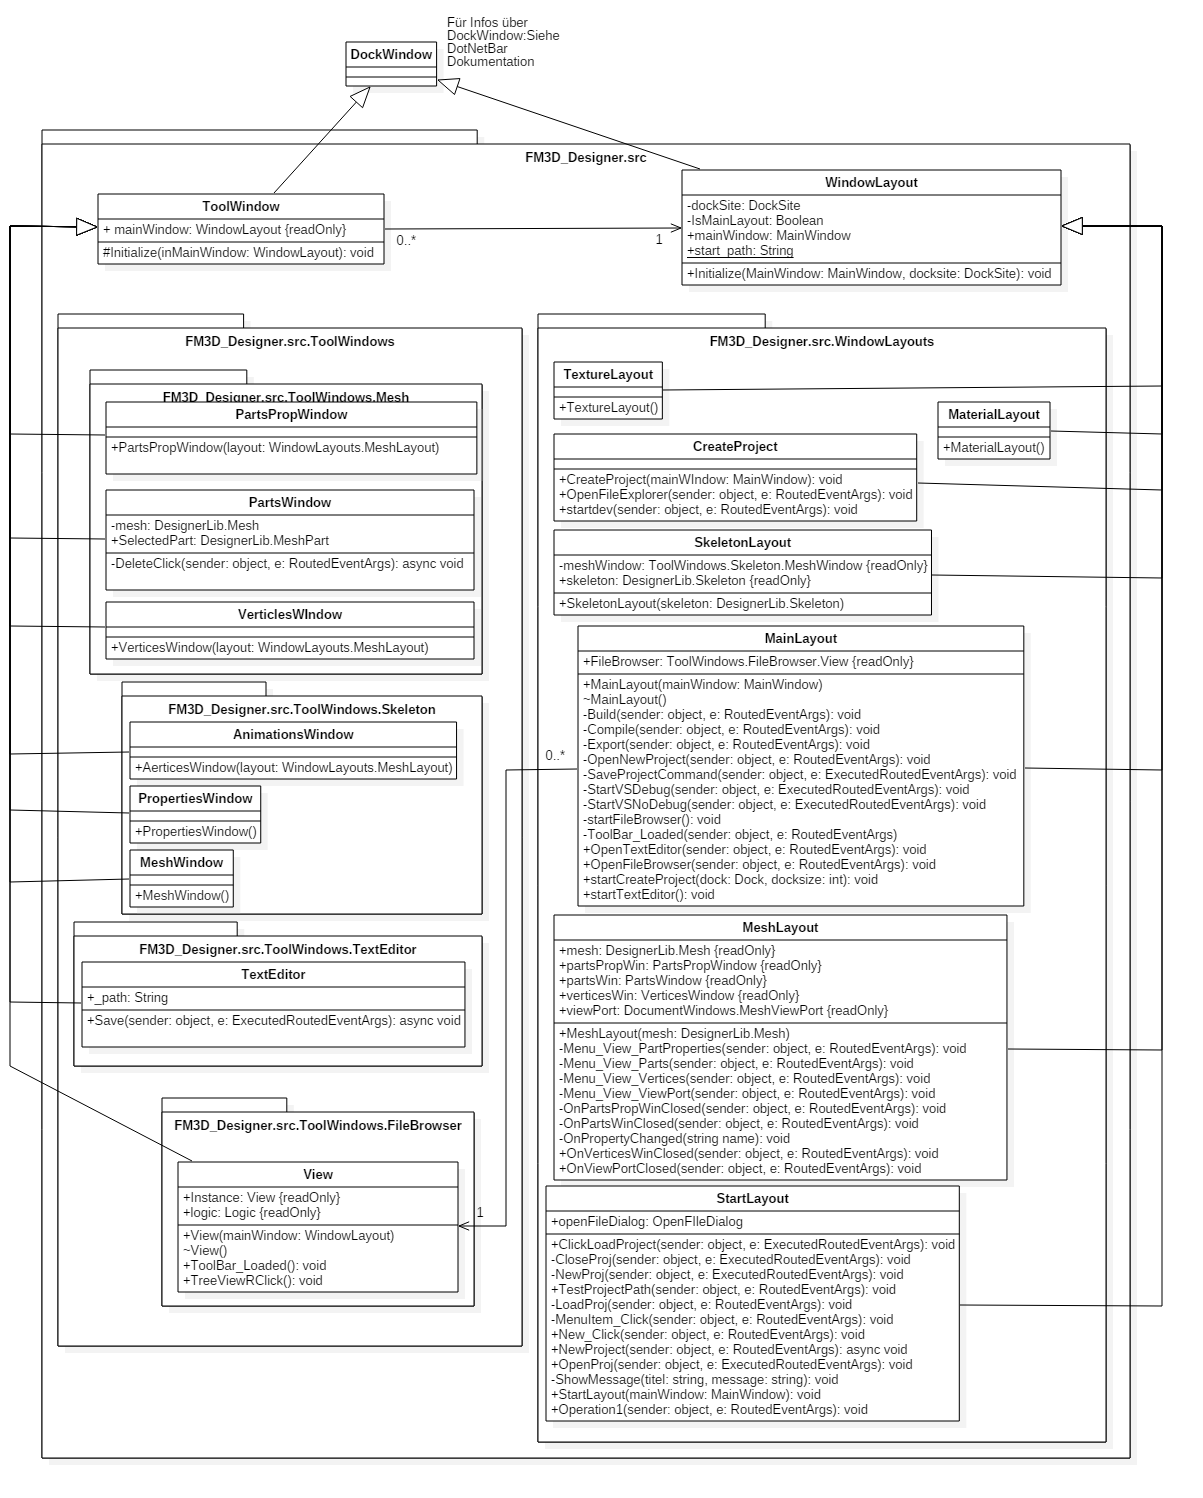
\includegraphics[width=1.2\textwidth]{03unserprogramm/Designer/Layouts.png}
		\caption{Fenster-Klassen}\label{windowclass}
	\end{center}
\end{figure}

\begin{figure}
	\begin{center}
		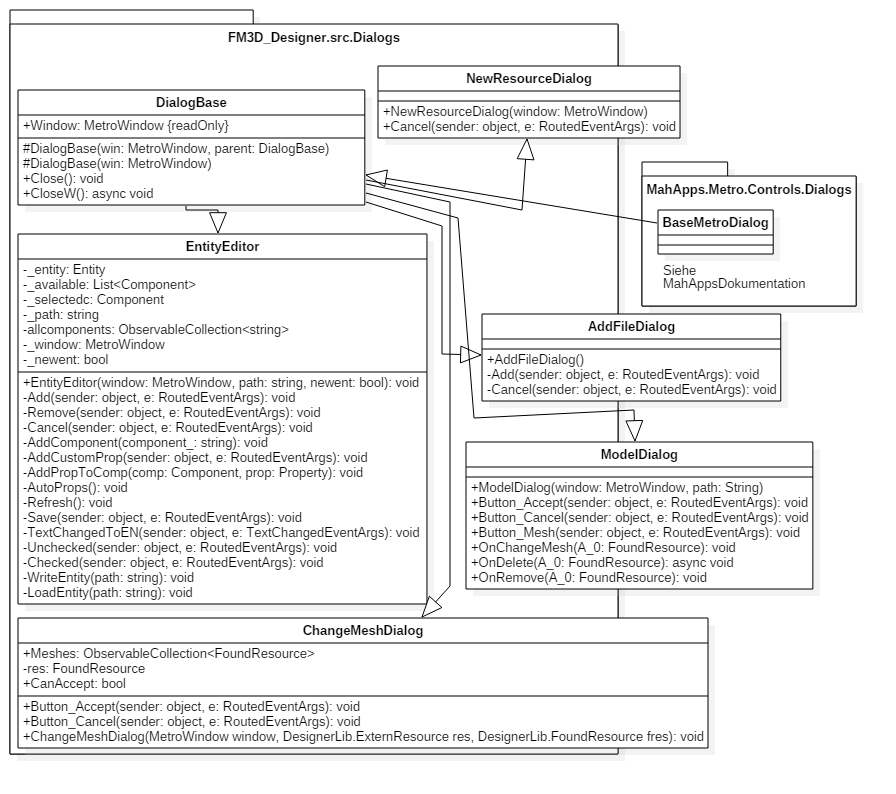
\includegraphics[width=\textwidth]{03unserprogramm/Designer/Dialogs.png}
		\caption{Dialog-Klassen}\label{dialogclass}
	\end{center}
\end{figure}

\subsection{Layouts}
\subsubsection{StartLayout}
\label{startlayout}
Das Start-Layout des Designers bietet dem Nutzer die Option ein Projekt in den Designer zu laden oder ein neues zu erstellen. Möchte man nun eines erzeugen, so wird man auf einen neuen Reiter gewiesen, in dem man nun Einstellungen bezüglich des zu erstellenden Projektes tätigen kann. Rechts davon befindet sich ein Text mit einem kurzen Anweisungstext zu dem Programm. Darunter ist ein Internet-Browser eingebunden, welcher die letzten Änderungen des Programmes anzeigt.

\subsubsection{CreateProjekt}
Nachdem man auf einen Nebenreiter des Startlayouts geleitet wurde, kann der User einen Pfad bestimmen in dem das Projekt geladen werden soll. Im vom User angegebenen Pfad werden jetzt zwei Ordner angelegt: Einen für die Projektdateien und einen für die C++ Dateien. 
In den Ordner der C++ Dateien wird nun ein VisualStudio-Projekt-Template erstellt, welches ein Projekt für das Spiel abbildet. Zu diesem wird eine "'fm3D.xml"` Datei in dem selben Ordner generiert. In dieser stehen Informationen, welche später für die Pipe \ref{pipe} benötigt werden. Darunter der Dateiname, Der Projektmappenname und die Pipe-ID.
Nun wird die Projektdatei in Form von einer XML-Datei mit der Endung "'.fmproj"` erzeugt. Diese wird beim Start der FM3D-Designer-Entwicklungsumgebung geladen und später in der \textit{TreeView} des \textit{File-Browsers} dargestellt.

\subsubsection{MainLayout}
\label{mainlayout}
Nachdem nun ein Projekt erstellt oder geöffnet und geladen wurde, wird der User auf das "'Main-Layout"` geleitet. Dort werden mit dem Start ein Texteditor und ein File-Browser in andockbaren Childfenstern geöffnet. In dem Kontextmenü des Programmes kann der User nun zwischen vier verschiedenen Reitern auswählen. Neben jeder Option werden zudem -falls Verfügbar- Tastenkürzel angezeigt. 
In dem ersten Reiter "'File"` kann der User entweder ein neues Projekt erstellen oder das aktuelle speichern. 
Im zweiten Kontextmenüitem sind die Operationen aufrufbar, welche für die Kommunikation mit der Extension (\ref{extension}) über die Pipe(\ref{pipe}) benötigt werden. Diese Optionen sind auch in Icons unter dem Kontextmenü abgebildet, um dem User ein schnelles arbeiten zu ermöglichen. Im dritten Kontextmenüitem kann man nun die verschiedenen andockbaren Fenster auswählen. Im vierten und letzten sind Informationen zum Entwicklerteam und über dieses Projekt zu finden.

\subsection{ToolWindows}
\subsubsection{FileBrowser}
\label{filebrowser}
Im File-Browser wird die Ordnerstruktur des FM3D-Projektes in Form der \textit{Item}-Klasse (Siehe \cref{item}) abgebildet. Der Nutzer kann durch diesen File-Browser nun entweder Daten erstellen oder sich diese darstellen lassen. Entity-Dateien können durch den Entity-Editor grafisch betrachtet und editiert werden. Alle abgebildeten Dateien können zudem in einem im Designer implementierten Text-Editor mit den nötigsten Funktionen bearbeitet werden.

\subsubsection{TextEditor}
Der Texteditor ist ein Tool um Texte zu editieren.  Es verfügt über die wichtigsten Funktionen, die ein Text-Editor verfügen sollte. Jede dieser Funktionen sind über Tastenkürzel aufrufbar.
\begin{itemize}
	\item Speichern
	\item Undo/Redo (Rückgängig/Wiederherstellen)
	\item Copy/Cut (Kopieren/Ausschneiden)
	\item Paste (Einfügen)
	\item Delete (Löschen)
\end{itemize}

\subsubsection{Mesh}
\todo[inline]{idk}
\subsubsection{Skeleton-Tools}
\todo[inline]{idk}

\subsection{Dialogs}
\subsubsection{Model-Loader | Add Resource-Dialog}
Der Model-Loader ist dafür gedacht, um simpel Modelle in den Designer zu laden, um sie dann in der Engine weiter verwenden zu können. Die Modeldatei wird analysiert und die Daten werden in eine Datei in der Ordnerstruktur des Designers gespeichert.
%Durch die Exportfunktion im Designer kann man nun Code generieren lassen, der die Modelle im Designer verwenden kann 
\todo[inline]{!!!}

\subsubsection{Entity-Editor}
\label{entityeditor}
Der Entity-Editor wurde implementiert, um dem Nutzer das erstellen von Entities zu erleichtern. (Um den Aufbau der Entities erfahren siehe: \ref{entitysystem}). Der Nutzer gibt im Entity-Editor zunächst die Komponenten ein, die das zu erstellende Entity haben soll. Zu diesen Komponenten werden nun optional Standart-Properties bereitgestellt, die automatisch hinzugefügt werden können. Der User kann außerdem noch weitere, Benutzer spezifische Properties zu den Entities hinzufügen. Diese ganzen Daten werden nun in Form einer .xml Datei mit der Endung "'.ent"` im Projektordner gespeichert. Diese kann sich der Nutzer sowohl mit einem externen oder mit dem implementierten Texteditor im FM3D-Designer anschauen und wenn es ihm beliebt manuell verändern.


